\chapter{Introduction}
\lipsum[1-2]
\cite{latex1} \lipsum[1-2]

% Example 1
\clearpage
\newgeometry{left=4cm, right=2cm, top=3cm, bottom=3cm,
layoutwidth=29.7cm, layoutheight=21cm, layoutoffset=0cm,
textwidth=23.7cm,textheight=15cm}
\pdfpagewidth=29.7cm \pdfpageheight=21cm
\fancyheadoffset{0cm}

\lipsum[1]
\begin{table}[p]
\begin{center}

\begin{tabular}{|l|l|l|}
\hline
Year & Total (£)   & Total (\$) \\ \hline
2016 & £ 3,729.94  & \$ 403.87  \\ \hline
2017 & £ 1,905.11  & \$ 46.00   \\ \hline
2018 & £ 6,843.80  & \$ 325.00  \\ \hline
     & £ 12,478.85 & \$ 774.87  \\ \hline
\end{tabular}
\caption{Example Table}
\label{table:Example Table}
\end{center}
\end{table}

\clearpage
\newgeometry{left=4cm, right=2cm, top=3cm, bottom=3cm}
\pdfpagewidth=21cm \pdfpageheight=29.7cm

% Example 2
\clearpage
\newgeometry{left=4cm, right=2cm, top=3cm, bottom=3cm,
layoutwidth=29.7cm, layoutheight=42cm, layoutoffset=0in,
textwidth=23.7cm,textheight=36cm}
\pdfpagewidth=29.7cm \pdfpageheight=42cm
\fancyheadoffset{0cm}

\begin{figure}[p]
    \centering
    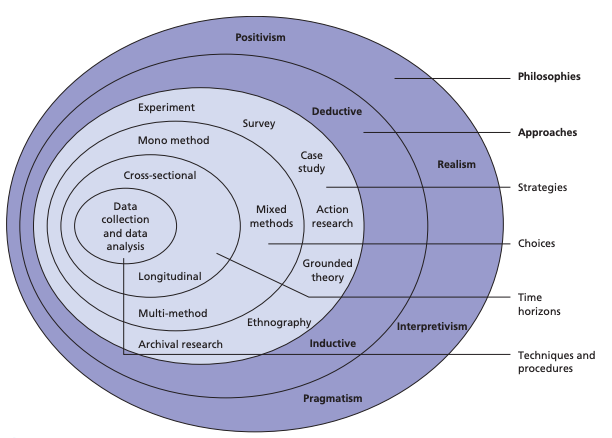
\includegraphics[width=0.8\textwidth]{ResearchOnion}
    \caption{The Research Onion}
    \label{fig:research-onion}
\end{figure}

\clearpage
\newgeometry{left=4cm, right=2cm, top=3cm, bottom=3cm}
\pdfpagewidth=21cm \pdfpageheight=29.7cm 